%%\documentclass[a4paper,12pt,oneside]{llncs}
\documentclass[11pt,letterpaper]{article}
\usepackage[right=2cm,left=3cm,top=2cm,bottom=2cm,headsep=0cm]{geometry}

%%%%%%%%%%%%%%%%%%%%%%%%%%%%%%%%%%%%%%%%%%%%%%%%%%%%%%%%%%%
%% Juego de caracteres usado en el archivo fuente: UTF-8
\usepackage{ucs}
\usepackage[utf8x]{inputenc}

%%%%%%%%%%%%%%%%%%%%%%%%%%%%%%%%%%%%%%%%%%%%%%%%%%%%%%%%%%%
%% Juego de caracteres usado en la salida dvi
%% Otra posibilidad: \usepackage{t1enc}
\usepackage[T1]{fontenc}

%%%%%%%%%%%%%%%%%%%%%%%%%%%%%%%%%%%%%%%%%%%%%%%%%%%%%%%%%%%
%% Ajusta maergenes para a4
%\usepackage{a4wide}

%%%%%%%%%%%%%%%%%%%%%%%%%%%%%%%%%%%%%%%%%%%%%%%%%%%%%%%%%%%
%% Uso fuente postscript times, para que los ps y pdf queden y pequeños...
\usepackage{times}

%%%%%%%%%%%%%%%%%%%%%%%%%%%%%%%%%%%%%%%%%%%%%%%%%%%%%%%%%%%
%% Posibilidad de hipertexto (especialmente en pdf)
%\usepackage{hyperref}
\usepackage[bookmarks = true, colorlinks=true, linkcolor = black, citecolor = black, menucolor = black, urlcolor = black]{hyperref}

%%%%%%%%%%%%%%%%%%%%%%%%%%%%%%%%%%%%%%%%%%%%%%%%%%%%%%%%%%%
%% Graficos 
\usepackage{graphics,graphicx}

%%%%%%%%%%%%%%%%%%%%%%%%%%%%%%%%%%%%%%%%%%%%%%%%%%%%%%%%%%%
%% Ciertos caracteres "raros"...
\usepackage{latexsym}

%%%%%%%%%%%%%%%%%%%%%%%%%%%%%%%%%%%%%%%%%%%%%%%%%%%%%%%%%%%
%% Matematicas aun más fuertes (american math dociety)
\usepackage{amsmath}

%%%%%%%%%%%%%%%%%%%%%%%%%%%%%%%%%%%%%%%%%%%%%%%%%%%%%%%%%%%
\usepackage{multirow} % para las tablas
\usepackage[spanish,es-tabla]{babel}

%%%%%%%%%%%%%%%%%%%%%%%%%%%%%%%%%%%%%%%%%%%%%%%%%%%%%%%%%%%
%% Fuentes matematicas lo mas compatibles posibles con postscript (times)
%% (Esto no funciona para todos los simbolos pero reduce mucho el tamaño del
%% pdf si hay muchas matamaticas....
\usepackage{mathptm}

%%% VARIOS:
\usepackage{slashbox}
\usepackage{verbatim}
\usepackage{array}
\usepackage{listings}
\usepackage{multirow}
\usepackage{pdfpages}
\usepackage{tabularx}


%% MARCA DE AGUA
%% Este package de "draft copy" NO funciona con pdflatex
%%\usepackage{draftcopy}
%% Este package de "draft copy" SI funciona con pdflatex
%%%\usepackage{pdfdraftcopy}
%%%%%%%%%%%%%%%%%%%%%%%%%%%%%%%%%%%%%%%%%%%%%%%%%%%%%%%%%%%
%% Indenteacion en español...
\usepackage[spanish]{babel}

\usepackage{listings}
% Para escribir código en C
% \begin{lstlisting}[language=C]
% #include <stdio.h>
% int main(int argc, char* argv[]) {
% puts("Hola mundo!");
% }
% \end{lstlisting}

\title{Cuestiones AC}
\author{Jesús Rodríguez Heras}

\begin{document}
\maketitle
\thispagestyle{empty}
\newpage

\tableofcontents
\newpage

\section{Contrastar SISD, SIMD y MIMD}
\subsection{SISD}
\noindent
Un computador SISD solo tiene un procesador (CPU), el cual unicamente tiene una unidad de control (UC) y una unidad de procesamiento (ALU).
\subsection{SIMD}
\noindent
Un computador SIMD solo tiene un procesador (CPU), el cual tiene una unidad de control (UC) y varias unidades de procesamiento (ALU).
\begin{center}
	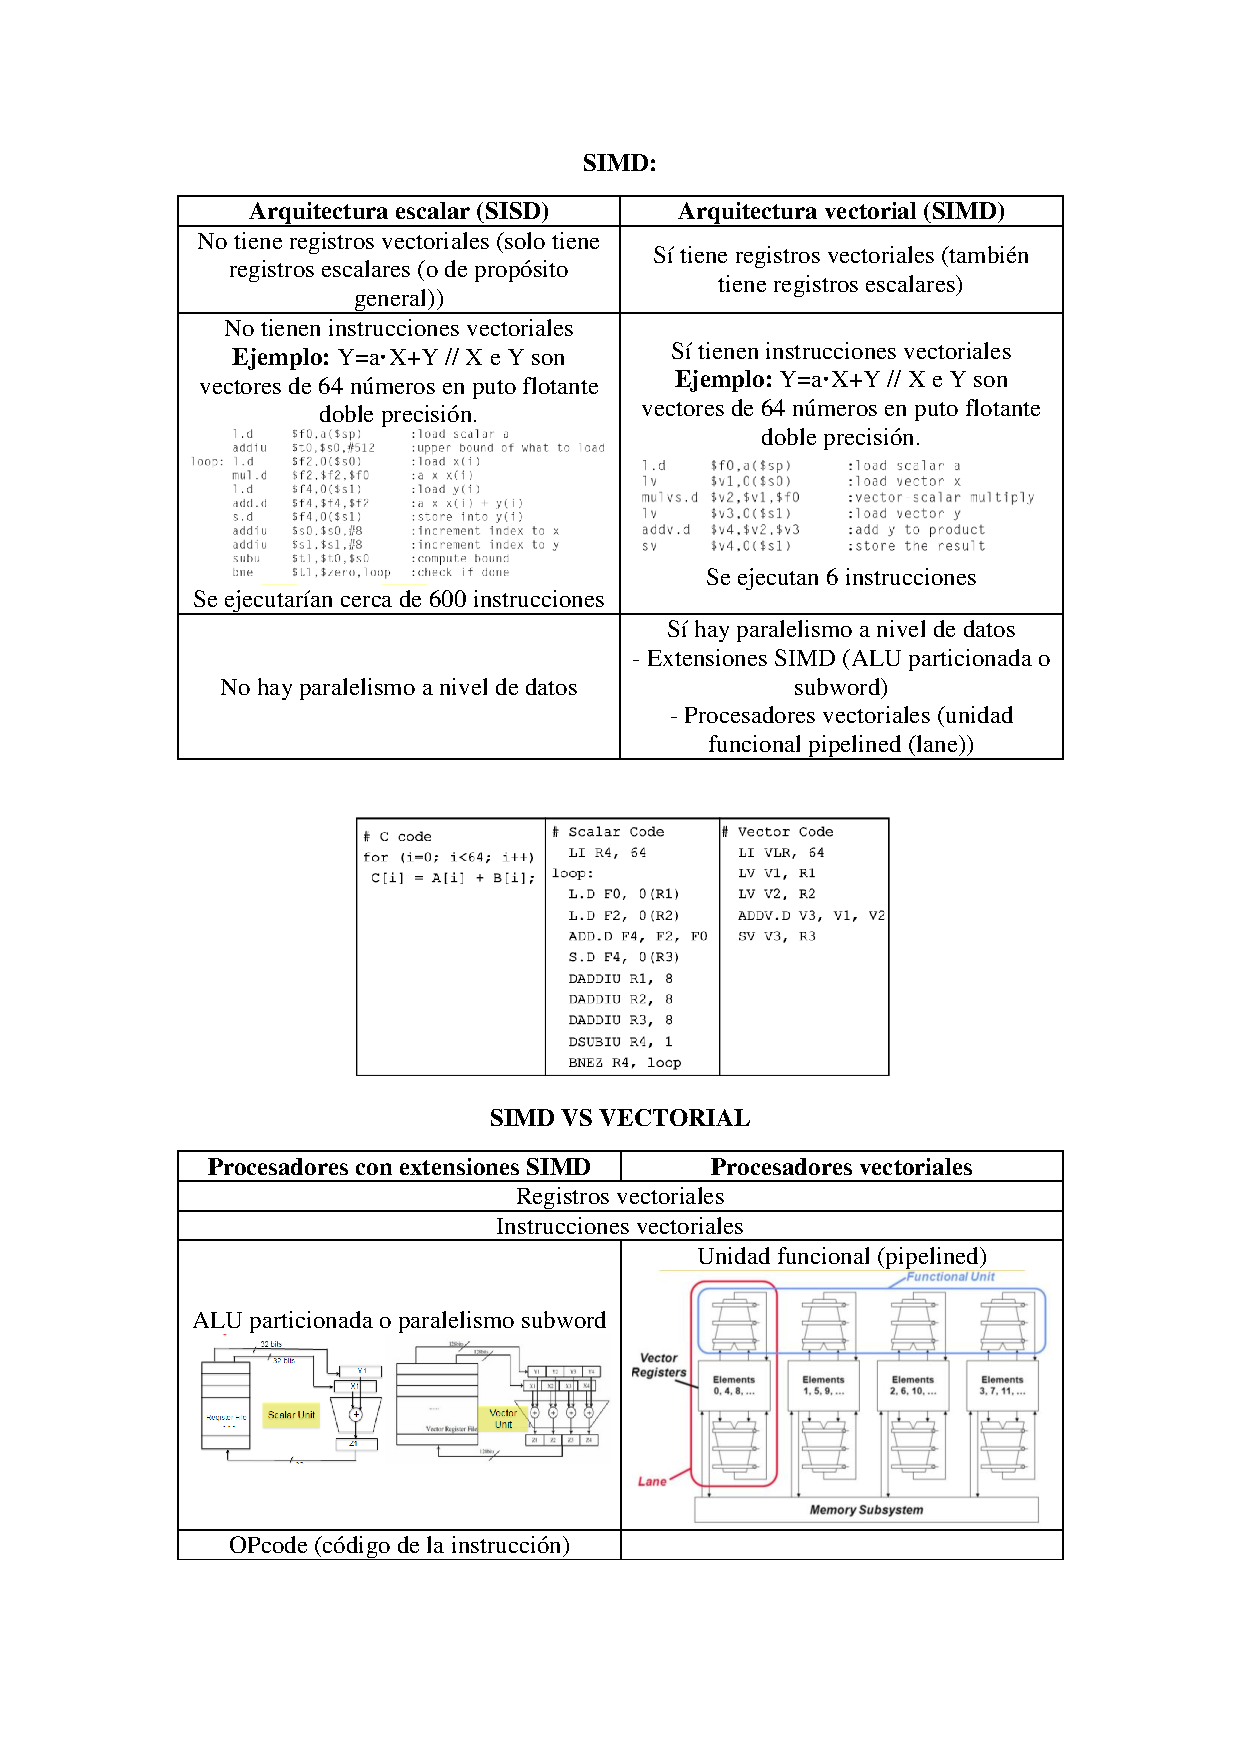
\includegraphics[scale=0.9]{SIMD.png}
\end{center}
\newpage
\noindent
Las extensiones SIMD implementan instrucciones para el manejo de múltiples datos y datos vectoriales o de coma flotante. Se implementa mediante una ALU particionada, lo que reduce el número de las operaciones que deben ser soportadas por el sistema y elimina los indicadores de excepciones.\\
La clasificación SIMD está compuesta de un grupo determinado de procesadores SISD, estos reciben una misma instrucción pero diferentes datos con los que operar, así se consigue un paralelismo a nivel de datos que permite realizar un único proceso. Esto es lo que ocurre en los procesadores multinúcleo, donde cada núcleo se comporta como un procesador.
\begin{center}
	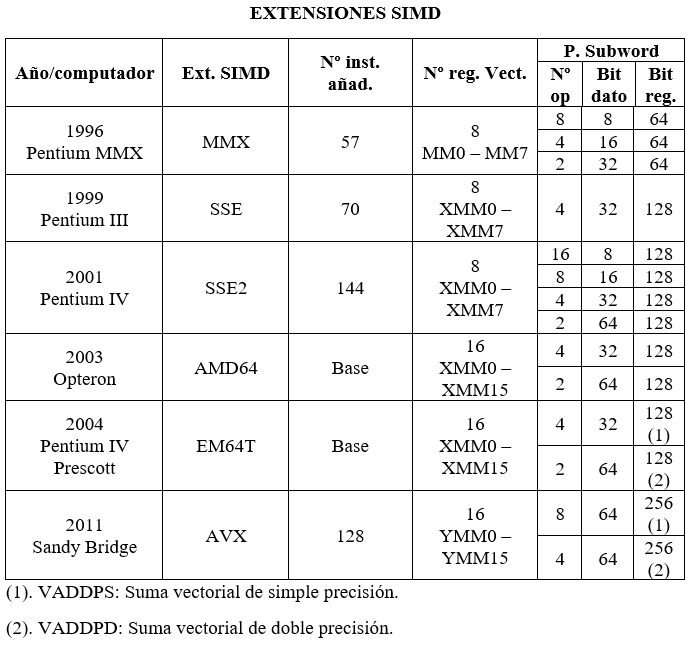
\includegraphics[scale=0.9]{ExtensionesSIMD.png}
\end{center}
\subsection{MIMD}
\noindent
Un computador MIMD tiene varios procesadores (CPU) y cada uno de ellos tiene su unidad de control (UC) y su unidad de procesamiento (ALU).\\
Dentro de los computadores MIMD podemos diferenciar dos tipos:
\newpage
\subsubsection{Memoria compartida (multiprocesadores)}
\noindent
Existe un único espacio de direcciones que es compartido por todos los procesadores y, normalmente, está formado por una sola computadora.\\
Un ejemplo de ello son los procesadores multinúcleo.
\subsubsection{Memoria distribuida (multicomputadores)}
\noindent
Cada procesador tiene su propio espacio de direcciones. Consta de un conjunto de computadoras conectadas entre sí por una red de comunicaciones que es percibido por el usuario como un solo sistema.\\
Un ejemplo de ello son los clusters y los grid.

\section{Arquitectura escalar vs Arquitectura vectorial}
\begin{center}
	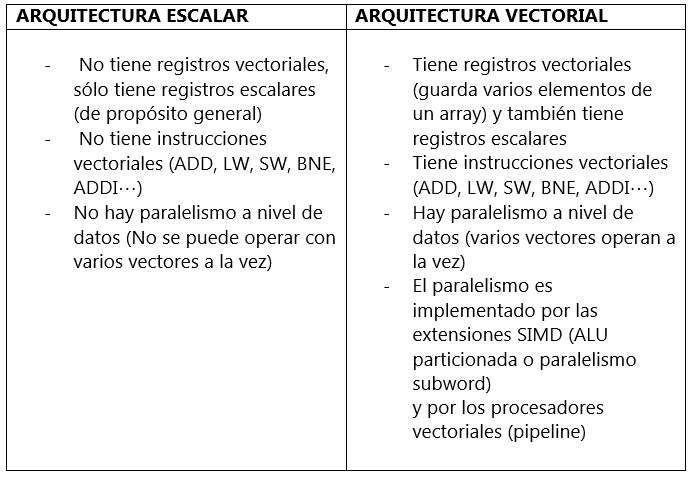
\includegraphics[scale=0.9]{EscalarVectorial.png}
\end{center}

\section{Arquitectura vectorial: Procesador con extensiones SIMD vs Procesador vectorial}
\noindent
La arquitectura vectorial es un esquema de microprocesadores cuya función está orientada a las operaciones con vectores.
\subsection{Procesador con extensiones SIMD}
\noindent
Un procesador con extensiones SIMD es un procesador escalar capaz de realizar las funciones de un procesador vectorial gracias a las extensiones SIMD (SSE, etc).
\subsection{Procesador vectorial}
\noindent
 Consta de una unidad escalar segmentada y una unidad vectorial. La unidad vectorial dispone de M registros vectoriales de N elementos y de unidades funcionales vectoriales que trabajan sobre los registros vectoriales, y un conjunto de registros escalares.

\section{Paralelismo subword}
\noindent
El paralelismo subword es la posibilidad de realizar varias operaciones simultaneas con datos de tamaño menor a una palabra.

\section{Caché directa}
\noindent
En la caché directa, un bloque procedente de memoria principal solo puede situarse en una posición determinada de la memoria caché. Esta posición está determinada por la dirección que tiene ese bloque en memoria principal. Las posiciones de la memoria caché se identifican con un índice. La etiqueta contiene la parte de la dirección que no aparece en el índice, es decir, la parte más significativa de la dirección.
\subsection{Funcionamiento}
\noindent
1.) El procesador está ejecutando la instrucción LW \$t0, 1101: cargar en el registro \$t0 el dato que está en la dirección de memoria 1101. Por tanto, el procesador tiene que acudir al sistema de memoria para obtener el dato.\\
2.) Comprueba si el dato está en el primer nivel de la jerarquía de memoria, es decir, en caché.\\
3.) Va al índice que coincide con la parte menos significativa de la dirección 1101 presente en la instrucción LW.\\
4.) Verifica si la etiqueta de ese índice coincide con la parte más significativa de la dirección 1101. Como coincide, se puede afirmar que el dato está en caché (ACIERTO). En caso de no coincidir, se puede afirmar que el dato no está en caché (FALLO) y habría que ir a memoria principal a buscarlo.


\section{Caché asociativa por conjuntos}
\noindent
La caché está dividida en conjuntos de bloques (vías).\\
Cada conjunto se identifica por un índice.\\
Un bloque de memoria principal solo puede ser situado en un conjunto concreto de la memoria caché asociativa por conjuntos, pero dentro de ese conjunto puede emplazarse en cualquier bloque (método aleatorio) o en el bloque que lleva más tiempo sin utilizarse (método LRU).
\subsection{Funcionamiento}
\noindent
1.) El procesador está ejecutando la instrucción LW \$t0, 1101: cargar en el registro \$t0 el dato que está en la dirección de memoria 1101. Comprueba si el dato está en caché. \\
2.) Va al índice y ve si coincide con la parte menos significativa de la dirección 1101 presente en la instrucción LW. \\
3.) Mira todas las etiquetas del conjunto en paralelo para verificar si hay alguna que coincida con la parte más significativa de la dirección 1101. Como hay una etiqueta que coincide, la petición de memoria acierta en caché. En caso contrario, se produce un fallo y hay que ir a memoria principal a buscar el dato.


\section{Contrastar cachés L1, L2 y L3}
\begin{center}
	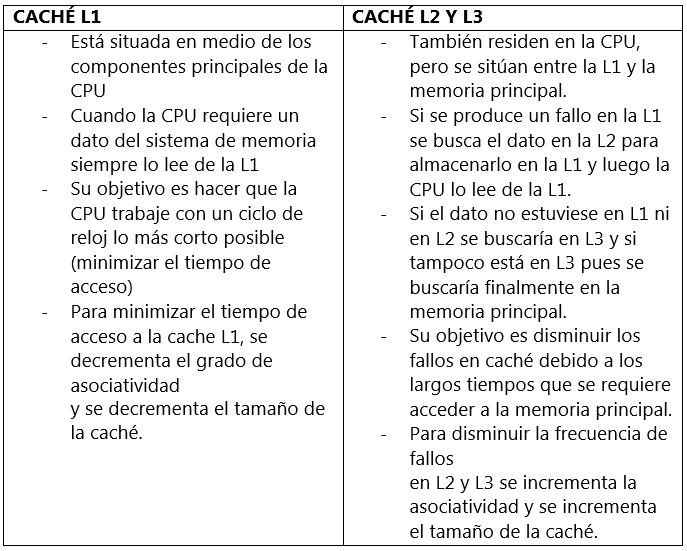
\includegraphics[scale=0.9]{Caches.png}
\end{center}
La caché L2 puede estar compartida entre todos los cores o ser exclusiva de cada core.

\section{ILP (paralelismo a nivel de instrucción)}
\noindent
Consiste en que la combinación de instrucciones de un mismo proceso que ejecuta un procesador puedan ser ordenadas de forma tal que, al ser procesadas a la vez (paralelamente), no afecten al resultado final del programa. La principal finalidad de dicho paralelismo es aumentar la velocidad y aprovechar al máximo las capacidades hardware del ordenador.
\subsection{Procesador segmentado (pipelined)}
\noindent
La técnica pipelined es una técnica en la que se separan por etapas el camino de las instrucciones para que instrucciones diferentes puedan alojarse en etapas diferentes.
\subsection{Procesador supersegmentado (profundidad del pipeline incrementada)}
\noindent
Es una técnica en la cual se segmentan las etapas de ejecución de una instrucción para que más instrucciones puedan ser ejecutadas consecutivamente.
\subsection{Procesador con ejecución múltiple}
\noindent
Podemos diferenciar dos tipos:
\subsubsection{Procesador superescalar (planificación dinámica)}
\noindent
Consiste en el duplicado de todos los componentes de una CPU para ejecutar dos instrucciones simultáneamente sin que estas visiten las mismas zonas del DIE.
\subsubsection{Procesador VLIW (planificación estática)}
\noindent
Se basa en las arquitecturas superescalares ya que ambas usan varias unidades funcionales o replican dichas unidades funcionales. Se caracteriza por tener pocas instrucciones pero su tamaño es muy grande (Very Long Instrucction Word). En cada instrucción se especifica el estado de todas las unidades funcionales del sistema, con el objetivo de simplificar el diseño del hardware al dejar todo el trabajo de planificar el código en manos del programador/compilador, en oposición a un procesador superescalar, en el que es el hardware en tiempo de ejecución el que planifica las instrucciones. VLIW=IA-64.\\
Cualquier mejora de la arquitectura implica un cambio en el juego de instrucciones (retrocompatibilidad nula).\\
No está orientado al uso de propósito general.

\section{ILP vs PLP}
\begin{center}
	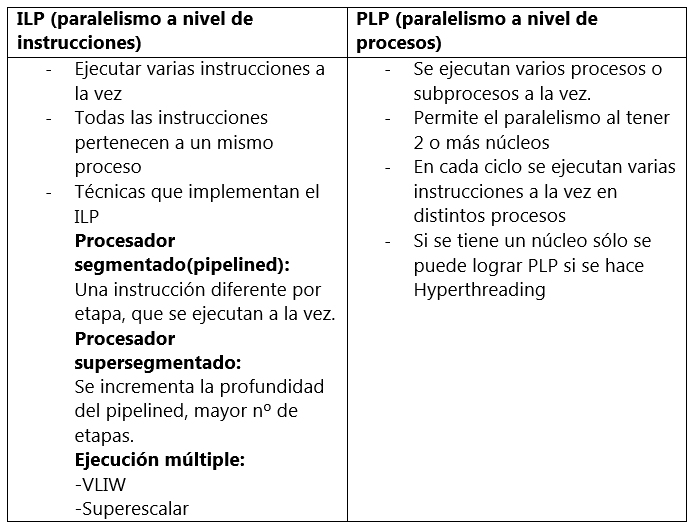
\includegraphics[scale=0.8]{ILPvsPLP.png}
\end{center}

\section{Hyperthreading}
\noindent
Es una técnica cuyo objetivo es conseguir PLP en un solo núcleo del procesador. Se simulan dos núcleos virtuales dentro de un núcleo físico.\\
Tenemos tres tipos:
\subsection{Grano fino}
\noindent
En cada instrucción se cambia de hilo (ejecución entrelazada de varios hilos). En la ejecución se salta los hilos parados en ese momento. Se cambia de hilo en cada ciclo de reloj.\\
\textbf{Ventaja:}  Cuando un hilo se para se pueden seguir ejecutando instrucciones de otros hilos por tanto se evitan que hayan muchas paradas largas o cortas.\\
\textbf{Desventaja: }Se pierde velocidad en la ejecución de un hilo individual porque un hilo que está listo para ejecutarse sin paradas se verá interrumpido por instrucciones de otros hilos.
\subsection{Grano grueso}
\noindent
El entrelazado de hilos sólo se realiza cuando hay una parada larga (Ejemplo: fallo de caché L2).\\
\textbf{Ventaja:} No se pierde velocidad en la ejecución de un hilo individual porque solamente se verá interrumpido el hilo por instrucciones de otros hilos si se produce una parada larga, en parada cortas no.\\
\textbf{Desventaja:} Se producen perdidas de prestaciones al no haber entrelazado en paradas cortas, cuando se produce una parada el pipelined se vacía y el nuevo hilo que se va a ejecutar debe volver a llenarlo antes de ser capaz de terminar las instrucciones, debido a este sobrecoste de llenado esta ejecución es más útil donde el tiempo de llenado del pipelined es muy pequeño en comparación al de parada.
\subsection{SMT}
\noindent
Su objetivo es explotar el paralelismo a nivel de hilos y a nivel de instrucciones a la vez.\\
No se conmutan sus hilos en cada ciclo, sino que están siempre ejecutando varias instrucciones de varios hilos. (El hardware determina las instrucciones a ejecutar y los registros asociados a cada hilo).\\
Las dependencias entre instrucciones se resuelven gracias a la planificación dinámica.
Resuelve el problema de los huecos en blanco por culpa de las dependencias.

\section{Contrastar ILP, PLP e Hyperthreading}
\begin{center}
	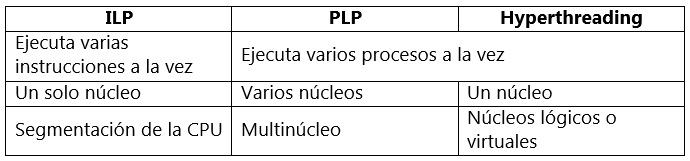
\includegraphics[scale=0.9]{ILPPLPHY.png}
\end{center}

\section{Elementos principales de un DIE}
\noindent
Es el chip que está en el procesador y que contiene toda su circuitería:
\begin{center}
	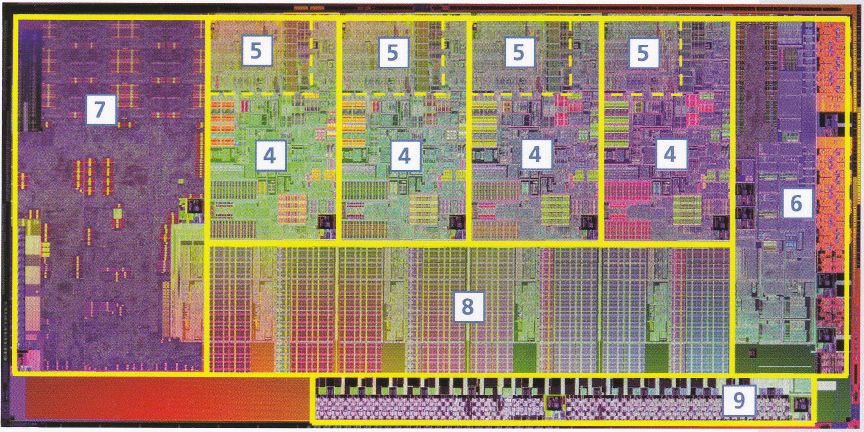
\includegraphics[scale=0.7]{DIE.png}
\end{center}
\subsection{Cachés L1 [4], L2 [5] y L3 [6]}
\noindent
Caché L1 está integrada cerca de la zona de los núcleos, cada núcleo tiene su propia caché L1, al igual que la caché L2 que está cerca y es una por núcleo.
La caché L3 sólo es una y se encuentra más alejada de los núcleos, es la caché más grande y lenta, es compartida por todos los núcleos del procesador.
\subsection{Núcleos [4]}
\noindent
Están justo en el centro del chip y tienen la unidad de control (UC) y la unidad aritmético-lógica (ALU).
\subsection{GPU (gráfica) [7]}
\noindent
La gráfica se encuentra integrada en el DIE también lo cual reduce el coste del PC y beneficia la comunicación entre el procesador gráfico y el procesador principal.
\subsection{Socket}
\noindent
Cuenta con miles de contactos para dar alimentación y realizar las comunicaciones con el resto del ordenador.
\subsection{Puente Norte [8]}
\noindent
Es un chip cuya función principal es la de controlar el funcionamiento del bus del procesador, la memoria y el puerto AGP o PCI-Express. De esa forma, entre la placa madre y los principales componentes de la PC.
\subsection{Interfaz de la memoria RAM [9]}
\noindent
Bus que conecta los zócalos de la memoria RAM con el controlador de memoria interno.

\newpage
\section{Tick-Tock y familias de procesadores}
\noindent
Es un modelo adoptado por Intel en el que se asocia cada “tick” con una mejora de la tecnología que representa una evolución en dicha tecnología (tamaño del procesador en nanómetros) y cada “tock” representa una mejora de la arquitectura (juegos de instrucciones).
\begin{center}
	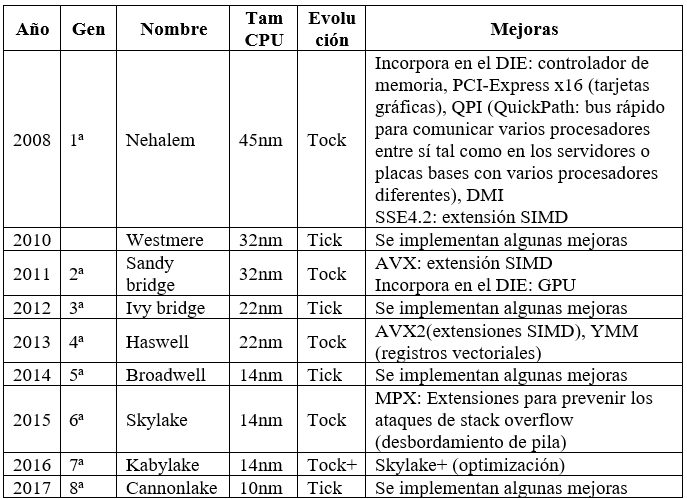
\includegraphics[scale=0.9]{TickTock.png}
\end{center}

\section{RISC vs CISC}
\begin{center}
	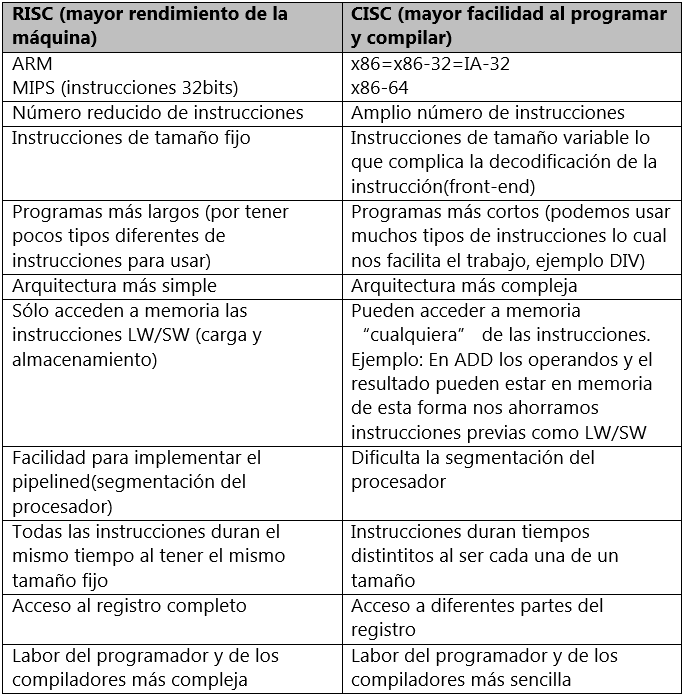
\includegraphics[scale=0.9]{RISCvsCISC.png}
\end{center}
\end{document}